%%%%%%%%%%%%%%%%%%%%%%%%%%%%%%%%%%%%%%%%%
% Beamer Presentation
% LaTeX Template
% Version 1.0 (10/11/12)
%
% This template has been downloaded from:
% http://www.LaTeXTemplates.com
%
% License:
% CC BY-NC-SA 3.0 (http://creativecommons.org/licenses/by-nc-sa/3.0/)
%
%%%%%%%%%%%%%%%%%%%%%%%%%%%%%%%%%%%%%%%%%

%----------------------------------------------------------------------------------------
%	PACKAGES AND THEMES
%----------------------------------------------------------------------------------------

\documentclass{beamer}

\mode<presentation> {

% The Beamer class comes with a number of default slide themes
% which change the colors and layouts of slides. Below this is a list
% of all the themes, uncomment each in turn to see what they look like.

%\usetheme{default}
%\usetheme{AnnArbor}
%\usetheme{Antibes}
%\usetheme{Bergen}
%\usetheme{Berkeley}
%\usetheme{Berlin}
%\usetheme{Boadilla}
%\usetheme{CambridgeUS}
%\usetheme{Copenhagen}
%\usetheme{Darmstadt}
%\usetheme{Dresden}
%\usetheme{Frankfurt}
%\usetheme{Goettingen}
%\usetheme{Hannover}
%\usetheme{Ilmenau}
%\usetheme{JuanLesPins}
%\usetheme{Luebeck}
\usetheme{Madrid}
%\usetheme{Malmoe}
%\usetheme{Marburg}
%\usetheme{Montpellier}
%\usetheme{PaloAlto}
%\usetheme{Pittsburgh}
%\usetheme{Rochester}
%\usetheme{Singapore}
%\usetheme{Szeged}
%\usetheme{Warsaw}

% As well as themes, the Beamer class has a number of color themes
% for any slide theme. Uncomment each of these in turn to see how it
% changes the colors of your current slide theme.

%\usecolortheme{albatross}
%\usecolortheme{beaver}
%\usecolortheme{beetle}
%\usecolortheme{crane}
%\usecolortheme{dolphin}
%\usecolortheme{dove}
%\usecolortheme{fly}
%\usecolortheme{lily}
%\usecolortheme{orchid}
%\usecolortheme{rose}
%\usecolortheme{seagull}
%\usecolortheme{seahorse}
%\usecolortheme{whale}
%\usecolortheme{wolverine}

%\setbeamertemplate{footline} % To remove the footer line in all slides uncomment this line
%\setbeamertemplate{footline}[page number] % To replace the footer line in all slides with a simple slide count uncomment this line

%\setbeamertemplate{navigation symbols}{} % To remove the navigation symbols from the bottom of all slides uncomment this line
}
\usepackage[utf8]{inputenc}
% \usepackage[english]{babel}

\usepackage{graphicx} % Allows including images
\usepackage{booktabs} % Allows the use of \toprule, \midrule and \bottomrule in tables

%----------------------------------------------------------------------------------------
%	TITLE PAGE
%----------------------------------------------------------------------------------------

\title[xx]{Metodo Spatio-temporal para la detección y registro de acciones humanas en video de poca resolucion. } % The short title appears at the bottom of every slide, the full title is only on the title page
\subtitle{}

\author[Autores]{
\small{presented by} 
\newline \normalsize {Luigy Machaca Arcana} }  % Your name
\institute[UNSA] % Your institution as it will appear on the bottom of every slide, may be shorthand to save space
{
Universidad Nacional de San Agustín\\ % Your institution for the title page
\medskip
%\textit{-----------} % Your email address
}
\date{\today} % Date, can be changed to a custom date

\begin{document}

\begin{frame}
\titlepage % Print the title page as the first slide
\end{frame}

\begin{frame}
\frametitle{Overview} % Table of contents slide, comment this block out to remove it
\tableofcontents % Throughout your presentation, if you choose to use \section{} and \subsection{} commands, these will automatically be printed on this slide as an overview of your presentation
\end{frame}

%----------------------------------------------------------------------------------------
%	PRESENTATION SLIDES
%----------------------------------------------------------------------------------------

%------------------------------------------------
\section{Introduction}
%------------------------------------------------



\begin{frame}
\frametitle{Introduction}
\begin{itemize}
\item El reconocimiento de acciones humanas sobre vídeo - visión artificial, 
\item Ha madurado lo suficiente.
\item La comprensión de la imagen es una tarea de importancia primordial para una amplia gama de aplicaciones prácticas.
\item un análisis de escena, que consiste en etiquetar cada píxel de la imagen con la categoría del objeto al que pertenece.
\end{itemize}
\end{frame}


\begin{frame}
\frametitle{Introduction}
\begin{itemize}
\item Un ejemplo, es el artículo de Yan lecun (2013) "La comprensión de la imagen es una tarea de importancia primordial para una amplia gama de aplicaciones prácticas. Un paso importante para entender una imagen es realizar un etiquetado de escena completa, también conocido como un análisis de escena, que consiste en etiquetar cada píxel de la imagen con la categoría del objeto al que pertenece."
\end{itemize}
 \begin{figure}
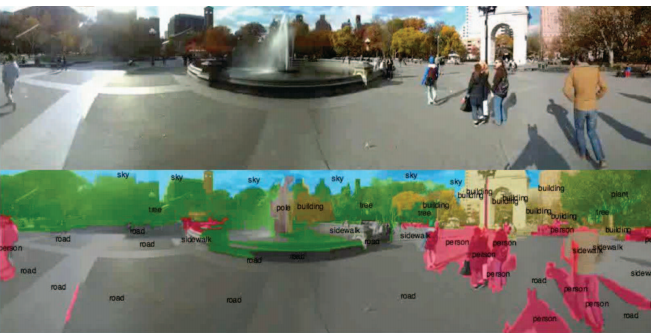
\includegraphics[width=0.8\linewidth]{img2/mccn.png}
\end{figure}

\end{frame}


\begin{frame}
\frametitle{Introduction}
\begin{itemize}
\item sparse techniques (Lucas-Kanade )

\item  dense techniques process all the pixels ( Poppe (2010)  describe los principales enfoques existentes para etiquetar acciones humanas sobre secuencias de vídeo 
)
\end{itemize}

\end{frame}






\begin{frame}
\frametitle{Introduction}
\begin{itemize}
\item  dense techniques process all the pixels
\end{itemize}
\begin{figure}
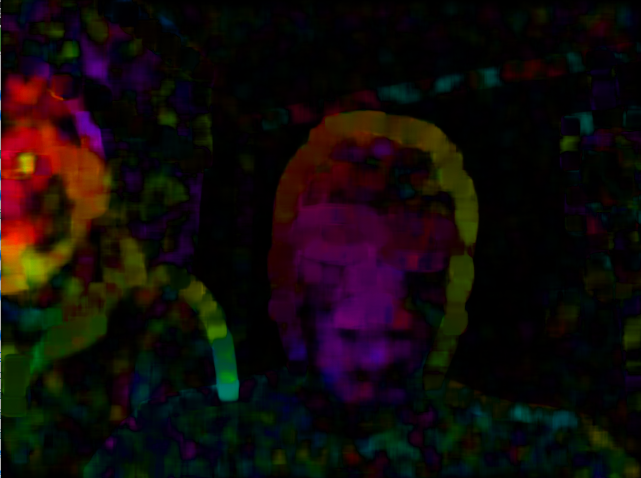
\includegraphics[width=0.8\linewidth]{img2/Dense_optical_flow_by_HSV_color_image.png}
\end{figure}

\end{frame}


\begin{frame}
\frametitle{Introduction}
\begin{itemize}
\item  dense techniques process all the pixels
\end{itemize}

\begin{figure}
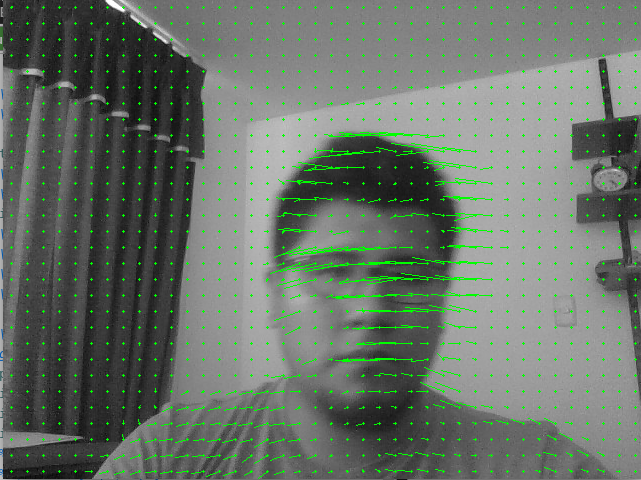
\includegraphics[width=0.8\linewidth]{img2/Dense_optical_flow_by_lines.png}
\end{figure}


\end{frame}




\begin{frame}
\frametitle{Introduction}
\begin{itemize}
\item Lucas-Kanade 
\begin{figure}
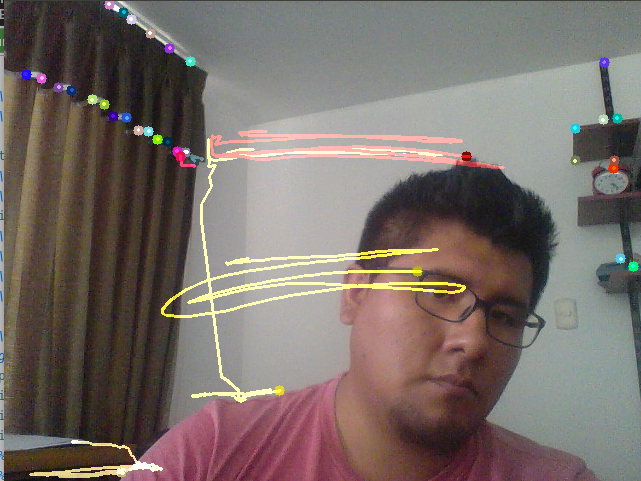
\includegraphics[width=0.8\linewidth]{img2/Lucas-Kanade_method.png}
\end{figure}
\end{itemize}


\end{frame}




\begin{frame}
\frametitle{Introduction}
\begin{itemize}
\item ¿Hay suficiente información spatio-temporal en un video para adquirir conocimiento sobre diferentes movimientos?
\end{itemize}

\end{frame}


\begin{frame}
\frametitle{Introduccion}
¿Hasta qué punto nosotros podemos capturar, representar y codificar toda la información de un video a un bajo costo computacional en tiempo real?


\begin{figure}
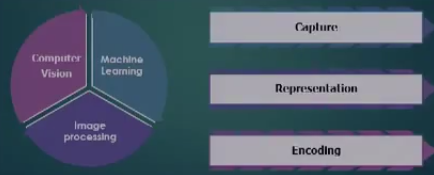
\includegraphics[width=0.8\linewidth]{img2/Selection_016.png}
\end{figure}

\end{frame}



%------------------------------------------------
\section{Porque los fenomenos spatio-temporal son tan importantes?
}
%------------------------------------------------

\begin{frame}	
\frametitle{Porque los fenomenos spatio-temporal son tan importantes?
}

\begin{itemize}
\item debido a que en una secuencia de imagenes (video), tenemos toda la información en estos pixeles.
\item tenemos una informacion especial en las distribuciones de los pixeles.
\item temporal information: cada píxel de un frame está relacionado con algún pixel del siguiente frame
\item si logramos relacionar estos píxeles, podremos por ejemplo: human action recognition
 
\end{itemize}
\begin{figure}
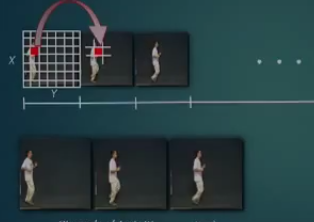
\includegraphics[width=0.4\linewidth]{img2/Selection_017.png}
\end{figure}

\end{frame}


\begin{frame}
\frametitle{¿Que podemos hacer con la computación visual?}
 
\begin{itemize}
\item \textbf{vision-based human recognition} es el proceso de etiquetado de secuencias de imágenes con etiquetas de acción.
	 \begin{itemize}
	 \item recognition, motion analysis, tracking, imagen registration
 
	 \end{itemize}
\item Es posible hacer aplicaciones de este tipo en tiempo real?
	\begin{itemize}
	\item ejemplo: puntajes en deportes
	\item content based video retrieval: 
		búsqueda de un video que contenta la misma información visual.
 
	\end{itemize}
\end{itemize}
 
\begin{figure}
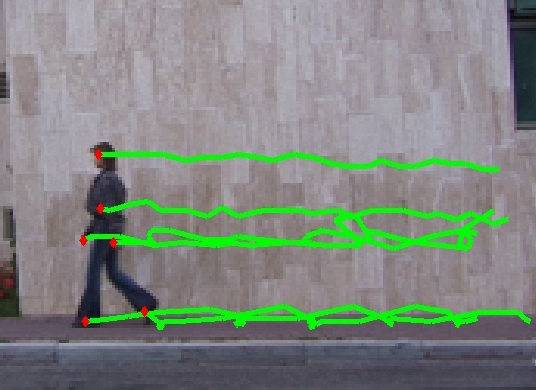
\includegraphics[width=0.2\linewidth]{img2/dariawalk.jpg}
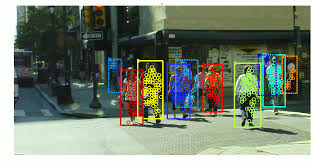
\includegraphics[width=0.4\linewidth]{img2/download.jpg}
 
\end{figure}
 
\end{frame}
 


 
\subsection{background}
\begin{frame}
\frametitle{¿Como obtenemos la información del video?}
 
\begin{itemize}
\item \textit{3d human body tracking with multiple cameras}
    \begin{itemize}
    \item En 3d, no puedes usar una solo cámara
     \item tiene un alto costo computacional
    \end{itemize}	
    \begin{figure}
    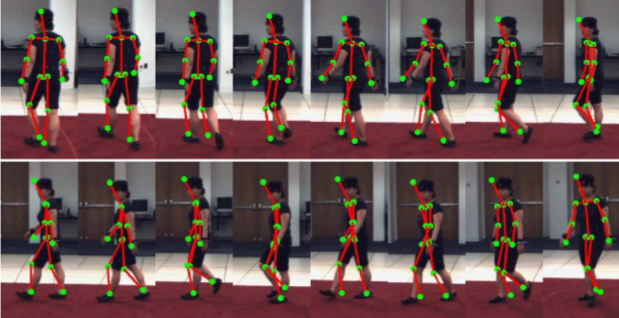
\includegraphics[width=0.4\linewidth]{img2/Selection_022.png} 
    \end{figure}
    
\item stick figure model with a nonparametric bayesian distribution
    \begin{itemize}
    \item no necesita informacion previa de un modelos, refiriéndose al modelo de movimiento.
    \end{itemize}

     \begin{figure}
     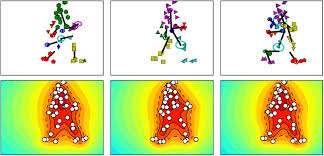
\includegraphics[width=0.4\linewidth]{img2/images.jpg} 
    \end{figure}

 \end{itemize}
\end{frame}
 


 
 
 
\begin{frame}
\frametitle{¿Como obtenemos la información del video?}
\begin{itemize}
	\item \textit{Learning Hierarchical Features for Scene Labeling}
    
     \begin{figure}
     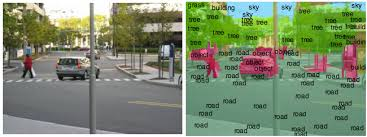
\includegraphics[width=0.4\linewidth]{img2/download__1_.jpg} 
    \end{figure}

 
	

\end{itemize}
 
\end{frame}
 
 
\section{algoritmo} 
 
 
 

 
 
\begin{frame}
\frametitle{¿Cuales son los problemas y las soluciones?}
 
\begin{itemize}
\item problema 1: atributos a gran escala del movimiento con los enfoques tradicionales.
	\begin{itemize}
      \item  nuevo enfoque spatio-temporal template (motion vector flow instance,MVFI)
      \item  reducción de dimensionalidad.
	\end{itemize}
\item problema 2: cómo retener información de temporal-connection en múltiples clasificaciones.
	\begin{itemize}
	\item trayectoria spatio-temporal 
	\item geometría de las curvas del spatio-temporal
	\item comparación de las propiedades de las curvas en mismas acciones.
 
	\end{itemize}
\end{itemize}
 
\end{frame}
 
  
 

\subsection{MVFI}
 
\begin{frame}
\frametitle{}
 
\begin{itemize}
\item spatio-temporal template (MVFI)
  \begin{itemize}
  \item dense optical flow: patrón de movimiento.
  \item flujo del vector movimiento.
  \item eigenvector: vectores que se fijan en dirección bajo una transformación lineal
  \item informacion
          \begin{itemize}
          \item magnitud de velocidad
          \item dirección de velocidad
          \end{itemize}
  \end{itemize}
\end{itemize}
  \begin{figure}
     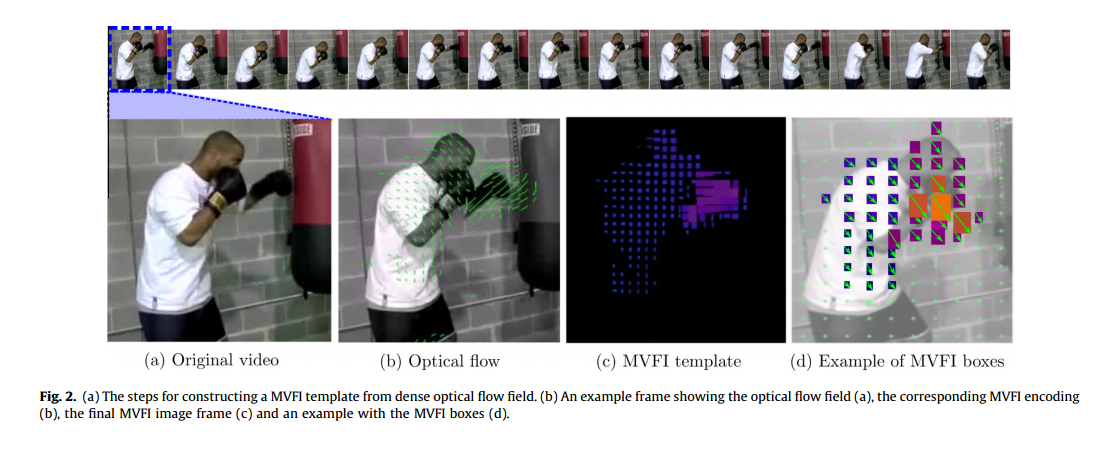
\includegraphics[width=0.8\linewidth]{img2/Selection_021.png} 
    \end{figure}
 
\end{frame}

\begin{frame}
\frametitle{Clasificación (machine learning)}
\begin{itemize}
\item Transformación un nuevo espacio para clasificarlos
	\begin{itemize}
      \item técnicas de reducción de dimensionalidad 
      \item principal component analysis(PCA) combinado con linear discriminant analysis(LDA)
	\end{itemize}
\item classification (k-nearest neighbors )

\end{itemize}
\end{frame}
 

\begin{frame}
\begin{figure}
 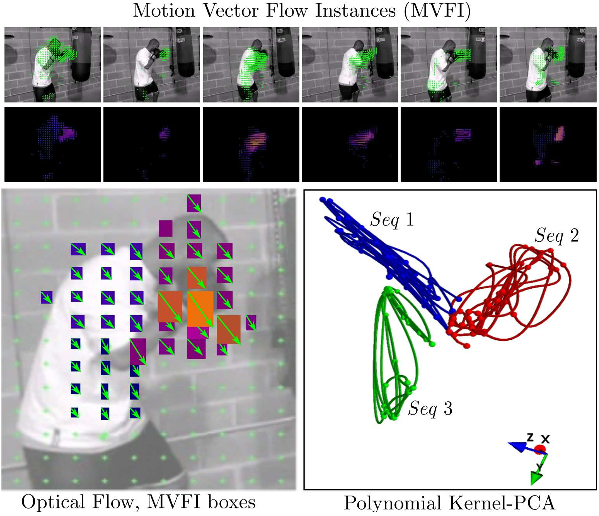
\includegraphics[width=0.8\linewidth]{img2/6-Figure2-1.png} 
\end{figure}
\end{frame}
 
 



%------------------------------------------------
\section{Objetivos}
%------------------------------------------------

\begin{frame}
\frametitle{Objetivos}
\begin{itemize}
\item aplicar una cnn para etapa clasificacion.
\item videos de baja resolucion. 
\item  
\end{itemize}
\end{frame}

%------------------------------------------------
\section{References}
%------------------------------------------------

\begin{frame}
\frametitle{References}
\footnotesize{
\begin{thebibliography}{99} 
    \bibitem[Alistarh, 2015]{p1} Gómez-Conde, Iván, and David N. Olivieri. "A KPCA spatio-temporal differential geometric trajectory cloud classifier for recognizing human actions in a CBVR system." Expert Systems with Applications 42.13 (2015): 5472-5490.
    
        \bibitem[K. Fraser, 2011]{p2}Gómez-Conde, Iván, et al. "Simple human gesture detection and recognition using a feature vector and a real-time histogram based algorithm." Journal of Signal and Information Processing 2.04 (2011): 279.
        
        \bibitem[Poppe,2010] {p3} Poppe, R. (2010). A survey on vision-based human action recognition. Image and vision computing, 28(6), 976-990.
        
        \bibitem[Yan LeCun,2013] {p4} Farabet, Clement, et al. "Learning hierarchical features for scene labeling." IEEE transactions on pattern analysis and machine intelligence 35.8 (2013): 1915-1929.
        
        
        
        
        
        
    
\end{thebibliography}
}
\end{frame}

%------------------------------------------------

\begin{frame}
\titlepage
\end{frame}

%----------------------------------------------------------------------------------------

\end{document}
